% ============================
\chapter{Un travail répétitif}
\label{chap:bcl}
% ============================

	Les ordinateurs révèlent tout leur potentiel dans leur capacité à répéter
	inlassablement les mêmes tâches.  Vous avez pu appréhender les boucles si
	vous avez utilisé \textit{studio.code.org} comme proposé dans la section
	\ref{codestudio} «~Ressources~» (cfr. p\,\pageref{codestudio})

	\marginicon{attention}
	\textbf{Conseil pédagogique.} 
	D’expérience, nous savons que ce chapitre est difficile à appréhender et
	qu'au fil des pages, la matière se complexifie.  C'est en restant assidus et
	aussidues~; en faisant les exercices et en demandant un retour sur ses
	solutions aux enseignants et enseignantes que l'on met toutes les chances de
	son côté. Si l'on se sent perdu, il ne faut pas hésiter à demander de
	l'aide. 

	\minitoc

% =======================================
\section{La notion de travail répétitif}
% =======================================

	Lorsque l'on veut (faire) effectuer un travail répétitif, 
	il faut indiquer deux choses~:
	\begin{itemize}
	\item le travail à répéter~;
	\item quand s’arrêter ou quand continuer ou encore,  combien de fois faire 
		le travail.
	\end{itemize}

	Examinons quelques exemples pour fixer notre propos.

	\paragraph{Exemple 1.} 
	Pour traiter des dossiers, nous pouvons dire 
	«~tant qu’il reste un dossier à traiter, le traiter~» 
	ou encore 
	«~traiter un dossier puis passer au suivant jusqu’à ce qu’il n’en 
	reste plus à traiter~».
	\begin{itemize}
	\item La tâche à répéter est~: «~traiter un dossier~».
	\item Quand continuer~: «~s’il reste encore un dossier à traiter~».
	\end{itemize}
	Nous aurions pu dire de manière semblable~:
	\begin{itemize}
	\item La tâche à répéter est~: «~traiter un dossier~».
	\item Quand s'arrêter~: «~dès qu'il n'y a plus de dossier à traiter~».
	\end{itemize}

	\paragraph{Exemple 2.}
	Pour calculer la cote finale de tous les étudiants et toutes les étudiantes,
	nous dirions quelque chose du genre 
	«~Pour tout étudiant, calculer sa cote~».
	\begin{itemize}
	\item 
		La tâche à répéter est~: «~calculer la cote d’un·e étudiant·e~».
	\item
		Combien de fois faire le travail~: «~autant qu'il y a d'étudiant·es~»

		Il faut le faire pour tous les étudiants et les étudiantes. Nous
		pourrions être plus précis et dire qu'il faut commencer au premier,
		passer à chaque fois au suivant et s'arrêter lorsque c'est terminé avec
		le dernier. 
	
\end{itemize}

	\paragraph{Exemple 3.}
	Pour afficher tous les nombres de 1 à 100, nous dirions~:
	«~Pour tous les nombres de 1 à 100, afficher le nombre~».
	\begin{itemize}
	\item
		La tâche à répéter est~: «~afficher un nombre~».
	\item 
		Nous indiquons qu'il faut le faire pour tous les nombres de 1 à 100. Il
		faut commencer à 1, passer au suivant et s'arrêter après avoir afficher
		100.
\end{itemize}
		
% ===================================================
\section{Une même instruction, des effets différents}
% ===================================================

	Comprenez bien que c’est toujours la même tâche qui est exécutée mais pas
	avec le même effet à chaque fois.  Ainsi, c'est un dossier qui est traité
	mais à chaque fois un différent~; c'est un nombre qui est affiché mais
	à chaque fois un différent. 
	
	Par exemple, la tâche à répéter pour afficher des nombres ne peut pas être
	\pc{\K{afficher} 1} ni \pc{\K{afficher} 2} ni\dots{} Par contre, on pourra
	utiliser l’instruction \pc{\K{afficher} nb} si on s’arrange pour que la
	variable \pc{nb} s’adapte à chaque passage dans la boucle.

	\begin{quote}
		\bfseries
		De façon générale,
		pour obtenir un travail répétitif,
		il faut trouver une formulation de la tâche
		qui va produire un effet différent à chaque fois.
	\end{quote}
	
	\subsection{Exemple - Afficher les nombres de 1 à 5}
	%===================================================
	
		Si nous voulions un algorithme qui affiche les nombres de 1 à 5
		sans utiliser de boucle, nous pourrions écrire~:

		\begin{langagenaturel}
			print 1\\
			print 2\\
			print 3\\
			print 4\\
			print 5\\
		\end{langagenaturel}	
		
		Ces cinq instructions sont proches mais pas tout-à-fait identiques. 
		En l’état, nous ne pouvons pas encore en faire une boucle%
		\footnote{%
			Vous vous dites peut-être que ce code est simple~;
			inutile d’en faire une boucle.
			Ce n’est qu’un exemple.
			Que feriez-vous s’il faillait afficher les nombres
			de 1 à 1000~?
		}~;
		il va falloir ruser.
		Nous pouvons obtenir le même résultat avec l’algorithme suivant~:

		\begin{minipage}{5cm}
			\begin{langagenaturel}
				nb = 1\\
				print nb\\
				nb = 2\\
				print nb\\
				nb = 3\\
				print nb\\
				nb = 4\\
				print nb\\
				nb = 5\\
				print nb\\
			\end{langagenaturel}
		\end{minipage}
		\quad ou encore \quad
		\begin{minipage}{5cm}
			\begin{langagenaturel}
				nb = 1\\
				print nb\\
				nb = nb + 1\\
				print nb\\
				nb = nb + 1\\
				print nb\\
				nb = nb + 1\\
				print nb\\
				nb = nb + 1\\
				print nb\\
			\end{langagenaturel}
		\end{minipage}
		
		Il est plus compliqué, mais cette fois les lignes 2 et 3 se répètent
		exactement.  D’ailleurs, la dernière ligne ne sert à rien d’autre qu’à
		obtenir cinq copies identiques.  Le travail à répéter est donc~:

		\begin{langagenaturel}
			print nb\\
			nb = nb + 1
		\end{langagenaturel}

		Cette tâche doit être effectuée cinq fois dans notre exemple.
		Il existe plusieurs structures répétitives
		qui vont se distinguer par la façon dont on va
		contrôler le nombre de répétitions.
		Voyons-les une à une%
		\footnote{%
			Nous ne verrons pas de structure de type
			\pc{répéter 5 fois\dots}
			Elle est simple à comprendre
			mais pas souvent adaptée au problème à résoudre.
		}.

\clearpage
%========================
\section{Le «~tant que~» (\textit{while})}
\index{tant que}\index{while}\index{boucles}
%========================
	
	Le «~\textbf{tant que}~» est une structure qui demande à l’exécutant de
	répéter une tâche (une ou plusieurs instructions) tant qu’une condition
	donnée est vraie.
	
	\begin{langagenaturel}
		tant que une certaine condition est vraie, répeter\\
			\tab une ou plusieurs actions\\
		fin tant que\\
		continuer l'algorithme 
	\end{langagenaturel}

	À la fin de chaque exécution des actions, la condition est retestée. Tant
	qu'elle est vraie les actions sont exécutées à nouveau. 

	Dans la grammaire du langage, cette instruction s'écrit~:
	
	\begin{grammaire}
		while ( \grammarrule{Expression} )
		    \grammarrule{Statement}
	\end{grammaire}
	
	\textit{Expression} est une expression booléenne comme nous l'avons vu (cf.
	section \ref{expression booléenne} p.~\pageref{expression booléenne}) et
	\textit{Statement} peut être une seule instruction ou un bloc
	d'instructions délimitées par des accolades.
	
	\begin{minipage}{7cm}
	L’organigramme ci-contre décrit  le déroulement de cette structure.  On
	remarquera que si la condition est fausse dès le début, la tâche n’est
	jamais exécutée.
	\end{minipage}
	\quad
	\begin{minipage}{7cm}
		\begin{tikzpicture}[node distance = 1.5cm, auto]
			\node[startstop] (start) {Start};
			\node[decision, below of=start, yshift=-1.3cm, text width=2cm]%
				(if1) {Condition true ?};
			\draw[arrow] (start) -- (if1);
			\node[process, below of=if1, yshift=-1.3cm] (pro1) {Instructions};
			\draw[arrow] (if1) -- node[anchor=south, left] {yes} (pro1);
			\draw[arrow] (pro1.west) 
				.. controls(-3,-3) 
				.. (if1);
			\node[startstop, below of=pro1, yshift=-1cm] (stop) {End};
			\draw[arrow] (if1.east) 
				.. controls(4,-4.5) 
				.. node[anchor=east] {no} (stop);
		\end{tikzpicture}	
	\end{minipage}

	
	\textbf{Remarques}

	Comme pour la structure \pc{if}, la \pc{condition} est une expression
	à valeur booléenne.  
	
	Dans ce type de structure, il faut qu’il y ait dans la
	séquence d’instructions du \pc{while} c'est-à-dire le bloc indenté au moins
	une instruction qui modifie une des composantes de la condition de telle
	manière qu’elle puisse devenir \textbf{fausse} à un moment donné. Dans le
	cas contraire, la condition reste indéfiniment vraie et la boucle va tourner
	sans fin, c’est ce qu’on appelle une \textbf{boucle infinie}.
	



	\subsection{Exemple - Afficher les nombres de 1 à 5}
	%===================================================

		Reprenons notre exemple d’affichage des nombres de 1 à 5.
		Pour rappel, la tâche à répéter est~:

		\begin{langagenaturel}
			print nb\\
			nb = nb + 1
		\end{langagenaturel}

		La condition va se baser sur la valeur de \pc{nb}.
		On continue tant que le nombre n’a pas dépassé 5.
		Ce qui donne (en n’oubliant pas l’initialisation de \pc{nb})~:

		\begin{minipage}{7cm}
			\begin{java}
public static void count5(){
	int nb = 1;
	while (nb <= 5){
		System.out.println(nb);
		nb = nb + 1;
	}
	System.out.println(
		"nb vaut: " + nb);
}				
			\end{java}
		\end{minipage}
		\quad
		\begin{minipage}{7cm}
			\begin{tabular}{|>{\centering\arraybackslash}m{6mm}
						|*{3}{>{\centering\arraybackslash}m{1.2cm}}|}
				\hline
				\rowcolor{black!40}
					\verb_#_  & nb & condition & affichage \\			
				\hline
					2 & indéfini & {} & {} \\
					3 & 1                    & {}   & {} \\
					4 & {\color{gray}$\mid$} & vrai & {} \\
					5 & {\color{gray}$\mid$} &      & 1  \\
					6 & 2                    & {}   & {} \\
					4 & {\color{gray}$\mid$} & vrai & {} \\
					5 & {\color{gray}$\mid$} &      & 2  \\
					6 & 3                    & {}   & {} \\
					4 & {\color{gray}$\mid$} & vrai & {} \\
					5 & {\color{gray}$\mid$} &      & 3  \\
					6 & 4                    & {}   & {} \\
					4 & {\color{gray}$\mid$} & vrai & {} \\
					5 & {\color{gray}$\mid$} &      & 4  \\
					6 & 5                    & {}   & {} \\
					4 & {\color{gray}$\mid$} & vrai & {} \\
					5 & {\color{gray}$\mid$} &      & 5  \\
					6 & 6                    & {}   & {} \\
					4 & {\color{gray}$\mid$} & faux & {} \\
					8 & {\color{gray}$\mid$} & {}   & {nb vaut 6} \\
				\hline
			\end{tabular}
		\end{minipage}

	\subsection{Exemple - Généralisation à n nombres}
	%===================================================

		Généraliser l'algorithme pour qu'il reçoive le nombre
		d'itérations en paramètres se fait simplement comme suit:
		
		\begin{java}
public static void count(int n){
	int i = 1;
	while (i <= n){
		System.out.println(i);
		i = i + 1;
	}
	System.out.println(
		"i vaut: " + i);
}				
	\end{java}


%====================
	\section{Le «~pour~» (\textit{for})}
	\index{pour}\index{for}
%====================
	
	Cette structure va plutôt indiquer \textbf{combien de fois} la tâche doit
	être répétée.  Cela se fait au travers d’une \textbf{variable de contrôle}
	dont la valeur va évoluer à partir d’une valeur de départ jusqu’à une valeur
	finale.

	\begin{langagenaturel}
		pour une variable allant d'une valeur de départ à une valeur finale\\
		\tab exécuter une ou plusieurs actions\\
		fin pour \\
		continuer l'algorithme 
	\end{langagenaturel}

	Ou, en étant un peu plus précis et en précisant un pas différent de 1~:

	\begin{langagenaturel}
		pour variable = début jusqu'à fin par pas\\
		\tab exécuter une ou plusieurs actions\\
		fin pour \\
		continuer l'algorithme 
	\end{langagenaturel}


	\begin{minipage}{7cm}
		\vspace*{5cm}

		Dans ce type de structure, \pc{début}, \pc{fin} et \pc{pas} peuvent
		être des constantes, des variables ou des expressions entières. 
		
		\vspace*{1cm}
		
		La boucle s’arrête lorsque la variable dépasse la valeur de \pc{fin}. 
		
		\vspace*{1cm}
		
		L'organigramme ci-contre illustre le fonctionnement d'une boucle
		\pc{for}. 
		
		\vspace*{5cm}
	\end{minipage}
	\quad
	\begin{minipage}{7cm}
		\vspace{-1cm}
		\begin{tikzpicture}[node distance = 1.5cm, auto]
			\node[startstop] (start) {Start};
			\node[process, below of=start] (pro0) {variable = début};
			\node[decision, below of=pro0, yshift=-1.3cm, text width=2cm]%
				(if1) {variable $\le$ fin ?};
			\draw[arrow] (start) -- (pro0);
			\draw[arrow] (pro0) -- (if1);
			\node[process, below of=if1, yshift=-1.3cm] (pro1) {Instructions};
			\draw[arrow] (if1) -- node[anchor=south, left] {yes} (pro1);
			\node[process, below of=pro1] (pro2) {variable = variable + pas};
			\draw[arrow] (pro2.west) 
				.. controls(-3,-3) 
				.. (if1);
			\draw[arrow] (pro1) -- (pro2);
			\node[startstop, below of=pro2, yshift=-1cm] (stop) {End};
			\draw[arrow] (if1.east) 
				.. controls(5.5,-5.5) 
				.. node[anchor=east] {no} (stop);
		\end{tikzpicture}	
		\vspace{-4cm}
	\end{minipage}


	Dans la grammaire du langage Java, l'instruction \pc{for} est
	un peu plus large que de dire qu'une variable parcourt les valeurs allant de \pc{début} à \pc{fin}. Voici sa grammaire (simplifiée).

	\begin{grammaire}
		\grammarrule{ForStatement:}
		    for ( \grammarrule{ForInit}; \grammarrule{Expression}; \grammarrule{ForUpdate})
		        \grammarrule{Statement}
	\end{grammaire}

	\begin{description}
		\item[ForInit] initialise la variable;
			
			Par exemple \pc{variable = début}.\\
			Il sera nécessaire de la déclarer.

		\item[Expression] est la condition de fin;

		\item[ForUpdate] est l'incrément, le passage à l'itération suivante;

			Par exemple \pc{variable = variable + pas}
	\end{description}
	
	Une utilisation simple et fréquente du \pc{pour} a cette forme~:
	
	\begin{java}
for (int i = début; i < fin; i = i + pas){
	// statement
}
	\end{java}
	
	Nous verrons plus loin des exemples plus généraux du \pc{for} et nous
	verrons également qu'il existe également un \textit{enhanced for} — appelé
	\textit{foreach} — permettant une écriture très simple pour le parcours de
	certaines collections. 



	\subsection{Exemples}
	%===================================================

		Reprenons notre exemple d’affichage des nombres de 1 à 5.  Voici la
		solution avec un \pc{\algorithmicfor} et le traçage correspondant.

		\begin{minipage}{80mm}
			\begin{java}
public static void countTo5({
	for (int nb=1; nb<= 5; nb = nb+1){
		System.out.printl(i);
	}
	System.out.println("nb n'existe plus");
}
			\end{java}
		\end{minipage}
		\qquad
		\begin{minipage}{45mm}
			\begin{tabular}{|>{\centering\arraybackslash}m{3mm}
						|>{\centering\arraybackslash}m{3mm}
						>{\centering\arraybackslash}m{6mm}
						>{\centering\arraybackslash}m{12mm}|}
				\hline
					\verb_#_  & nb & cond. & affichage \\			
				\hline
					3 & 1                    & vrai 		& {} \\
					4 & {\color{gray}$\mid$} &      		& 1  \\
					3 & 2                    & vrai 		& {} \\
					4 & {\color{gray}$\mid$} &      		& 2  \\
					3 & 3                    & vrai 		& {} \\
					4 & {\color{gray}$\mid$} &      		& 3  \\
					3 & 4                    & vrai 		& {} \\
					4 & {\color{gray}$\mid$} &      		& 4  \\
					3 & 5                    & vrai 		& {} \\
					4 & {\color{gray}$\mid$} &      		& 5  \\
					3 & 6                    & faux 		& {} \\
					6 & \verb_#_             & \verb_#_	& {nb n’existe plus} \\
				\hline
			\end{tabular}
		\end{minipage}

		Pour généraliser à $n$ nombres, nous pouvons écrire~:
		

		\begin{java}
public static void countToN(int n){
	for (int i = 1; i <= n; i = i + 1){
		System.out.println(i);
	}
}
		\end{java}

		\paragraph{Remarques} 
		\begin{itemize}
			
			\item En langage Java, l'indice de la boucle est souvent noté
				\pc{i}. 

			\item Lorsqu'il n'est pas explicitement demandé le contraire,
				l'indice d'une boucle commence à 0.  
		
\end{itemize}



	\subsection{Un pas négatif}
	%===================================================

		Le pas est parfois négatif, dans le cas d’un compte à rebours, par
		exemple.  Dans ce cas, la boucle s’arrête lorsque la variable prend une
		valeur plus petite que la valeur de \pc{fin} et il faut faire attention
		à bien formuler la condition.
		
		\textbf{Exemple}~: Compte à rebours à partir de n.

		\begin{java}
public static void countTo1(int n){
	for (int i = n; i > 0; i = i - 1){
		System.out.print(i);
	}
	System.out.println("Go !");
}
\end{java}

	\subsection{Remarques}
	%===================================================

	\begin{enumerate}
	
		\item Il faut veiller à la cohérence de cette structure. 
		
			Nous pouvons considérer pour nos algorithmes qu’au cas (à éviter) où
			\pc{début} est strictement supérieur à \pc{fin} et le \pc{pas} est
			positif, la séquence d’instructions n’est jamais exécutée (mais ce
			n’est pas le cas dans tous les langages de programmation~!). Idem si
			\pc{début} est strictement inférieur à \pc{fin} mais avec un
			\pc{pas} négatif.


			\marginicon{attention}
		\item Il est important de ne pas modifier les variables de contrôle
			\pc{début}, \pc{fin} ou \pc{pas} ni de modifier la \pc{variable} au
			sein de la boucle pour garder une boucle lisible.

	\end{enumerate}

		
	
		
	
	\subsection{Exemple -- Afficher uniquement les nombres pairs}
	%===========================================================

		Cette fois-ci, nous allons écrire une boucle affichant uniquement 
		les nombres \textbf{pairs} jusqu’à la limite $n$.
		
		\textbf{Exemple~:}
		Les nombres pairs de $1$ à $10$ sont~: $2$, $4$, $6$, $8$, $10$.
		
		Notez que $n$ peut être impair. 
		Si $n$ vaut $11$, l’affichage est le même que pour $10$.
		Avec un «~pour~», une solution est~:


		\begin{java}
public static void printOdd(int n){
	for (int i=2; i <= n; i = i + 2){
		System.out.println(i);
	}
}
		\end{java}



		
		
		
\pagebreak[4]
%===================================
\section{«~faire~–~tant que~»}
\index{do-while}
%===================================

	À l'inverse du «~tant~que~-~faire~» qui peut ne pas exécuter la séquence
	d'instructions si le test est faux dès le départ, il existe une structure
	qui exécutera au moins une fois la séquence d'instructions avant de tester
	la condition. Cette instruction peut-être~:

	\begin{itemize}
		\item «~faire~-~jusqu'à~ce~que~» ou ;
		\item «~faire~-~tant~que~».
	\end{itemize}
	
	Cette structure est très proche du «tant~que~-~faire~» à ceci près que le
	test est fait à la fin et pas au début.
 
	\begin{langagenaturel}
		faire\\
			\tab une ou plusieurs actions\\
		jusqu'à ce qu'une certaine condition soit vraie\\
		continuer l'algorithme 
	\end{langagenaturel}
	
	ou
	
	\begin{langagenaturel}
		faire\\
			\tab une ou plusieurs actions\\
		tant que une certaine condition est vraie\\
		continuer l'algorithme 
	\end{langagenaturel}
	
	En Java, c'est le second choix qui est retenu

	\begin{grammaire}
	    \grammarrule{DoStatement:}
	    do 
	        \grammarrule{Statement}
	    while ( \grammarrule{Expression} );
	\end{grammaire}


	\begin{minipage}[]{7cm}
	
		\vspace{2cm}
		Comme avec le tant-que, il faut que la séquence d’instructions comprise
		entre \pc{\K{faire}} et \pc{\K{tant que}} contienne au moins une
		instruction qui modifie la condition de telle manière qu’elle puisse
		devenir \textbf{vraie} à un moment donné pour arrêter l’itération.  Le
		schéma ci-contre décrit le déroulement de cette boucle. 
		\vspace{2cm}
		
	\end{minipage}
	\quad
	\begin{minipage}[]{7cm}
		\begin{tikzpicture}[node distance = 1.5cm, auto]
			\node[startstop] (start) {Start};
			\node[process, below of=start] (pro0) {instructions};
			\node[decision, below of=pro0, yshift=-1.3cm, text width=2cm]%
				(if1) {condition vraie ?};
			\draw[arrow] (start) -- (pro0);
			\draw[arrow] (pro0) -- (if1);
			\draw[arrow] (if1.east) 
				.. controls(5,-4)
				.. node[anchor=east] {yes} (pro0.east);
			\node[startstop, below of=if1, yshift=-1.6cm] (stop) {End};
			\draw[arrow] (if1) -- node[anchor=north, left, yshift=-0cm] {no} (stop);
		\end{tikzpicture}	
		\vspace{-2cm}
	\end{minipage}





	\subsection{Exemple}
	%===================================================

		Reprenons notre exemple d’affichage des nombres de 1 à 5.
		Voici la solution et le traçage correspondant.

		\begin{minipage}{6.8cm}
			\begin{java}
public static void count5(){
	int nb = 1;
	do {
		System.out.println(nb);
		nb = nb + 1;
	} while (nb <= 5);
	System.out.println("nb vaut " + nb);
}
			\end{java}
		\end{minipage}
		\quad
		\begin{minipage}{7.2cm}
			\begin{tabular}{|>{\centering\arraybackslash}m{3mm}
						|>{\centering\arraybackslash}m{.8cm}
						>{\centering\arraybackslash}m{1.6cm}
						>{\centering\arraybackslash}m{1.2cm}|}
				\hline
				\rowcolor{black!40}
					\verb_#_  & nb & condition & affichage \\			
				\hline
					2 & indéfini & {} & {} \\
					3 & 1                    & {}   & {} \\
					5 & {\color{gray}$\mid$} &      & 1  \\
					6 & 2                    & {}   & {} \\
					7 & {\color{gray}$\mid$} & vrai & {} \\
					5 & {\color{gray}$\mid$} &      & 2  \\
					6 & 3                    & {}   & {} \\
					7 & {\color{gray}$\mid$} & vrai & {} \\
					5 & {\color{gray}$\mid$} &      & 3  \\
					6 & 4                    & {}   & {} \\
					7 & {\color{gray}$\mid$} & vrai & {} \\
					5 & {\color{gray}$\mid$} &      & 4  \\
					6 & 5                    & {}   & {} \\
					7 & {\color{gray}$\mid$} & vrai & {} \\
					5 & {\color{gray}$\mid$} &      & 5  \\
					6 & 6                    & {}   & {} \\
					7 & {\color{gray}$\mid$} & faux & {} \\
					8 & {\color{gray}$\mid$} & {}   & {nb vaut 6} \\
				\hline
			\end{tabular}
		\end{minipage}

		\paragraph{Exercice} Tracer l'algorithme si l'instruction 2 est \pc{int
		nb = 10;}. 

%======================================
\section{Quel type de boucle choisir~?}
%======================================

	En pratique, il est possible d’utiliser systématiquement la boucle \pc{tant
	que} qui peut s’adapter à toutes les situations.  
	
	Cependant, il est plus clair d’utiliser la boucle \pc{pour} dans les cas où
	le nombre d’itérations est fixé et connu à l’avance. Par là, nous voulons
	dire que le nombre d’itérations est déterminé au début de la boucle.  
	
	La boucle \pc{faire-tant que} convient quant à elle dans les cas où le
	contenu de la boucle doit être parcouru au moins une fois, alors que dans
	\pc{tant que}, le nombre de parcours peut être nul si la condition initiale
	est fausse.  
	
	La figure fig.\ref{fig:boucle-choix} ci-dessous propose un récapitulatif.

	\begin{center}
		\begin{figure}[h]
			\centering
			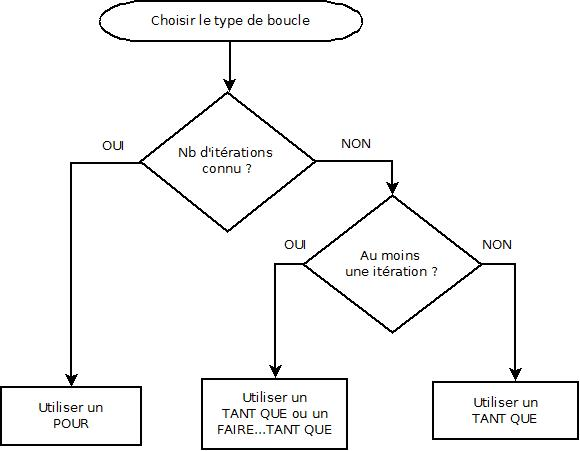
\includegraphics[width=.8\textwidth]{images/boucle-choixtype}
			\caption{Récapitulatif, choix d'une structure répétitive}
			\label{fig:boucle-choix}
		\end{figure}
	\end{center}




% ================================
\section{Exercices résolus}
% ================================

\subsection{Saisie des données par l'utilisateur}

	Il existe des problèmes où l’algorithme doit demander une série de valeurs
	à l’utilisateur pour pouvoir les traiter.  Par exemple, les sommer, en faire
	la moyenne, calculer la plus grande\dots
	
	Dans ce genre de problème, l'algorithme ou le programme stocke chaque valeur
	donnée par l’utilisateur dans une seule et même variable et la traite avant
	de passer à la suivante.  Prenons un exemple concret pour mieux comprendre.

	\begin{quote}
	Écrire un algorithme et un programme qui calcule et retourne 
	la somme d’une série de nombres donnés par l’utilisateur. 
	\end{quote}

	Il faut d’abord se demander comment l’utilisateur va pouvoir indiquer
	combien de nombres il faut additionner ou quand est-ce que le dernier nombre
	à additionner a été entré.  Voyons quelques possibilités.
	

	\subsubsection{Variante 1~: le nombre de valeurs est connu} 
	%-------------------------------------------------------	
	
		L’utilisateur indique le nombre de termes au départ.
		Ce problème est proche de ce qui a déjà été fait.
		
		En langage Java, l'habitude est de commencer à compter à partir de 0.
		Là où nous avons l'habitude de compter de $1$ à $n$, nous compterons
		toujours de $0$ à $n-1$. Plutôt que d'avoir comme condition de fin $i
		<= n - 1$, nous écrirons $i < n$.

		Une solution en Java peut-être~:

		\begin{java}
public static int sum(){
	int nValues;		// Nombre de valeurs à additionner
	int value;			// Terme de l'addition
	int sum = 0;		// Somme construite au fur et à mesure
	Scanner keyboard = new Scanner(System.in); // nécessite un import
	
	nValues = keyboard.nextInt();
	for  (int i = 0; i < nValues; i = i + 1){
		value = keyboard.nextInt();
		sum = sum + value;
	}
	return sum;
}
		\end{java}


		\paragraph{Remarque}

		Dans les exemples, nous utilisons des lectures au clavier très
		rudimentaires. Par exemple~:

		\begin{java}
value = keyboard.nextInt();			
		\end{java}

		Cette instruction, lorsqu'elle est exécutée, se traduit par un curseur
		qui clignote en attendant un nombre entier. Ce serait mieux de
		demander à l'utilisateur au préalable d'entrer un entier en lui écrivant
		un message. Plutôt comme suit~:

		\begin{java}
System.out.print("Entrer un entier: ");			
value = keyboard.nextInt();			
		\end{java}

		\texttt{nextInt} lit un entier au clavier. Si ce n'est pas un entier qui
		est entré… une erreur survient et le programme plante lamentablement.
		Pour éviter ceci, nous pouvons demander au programme de vérifier que
		l'utilisateur ou l'utilisatrice entre bien un entier, sinon, lui
		signaler. Justement la classe \texttt{Scanner} propose une méthode
		\texttt{hasNextInt}. Nous pourrions alors écrire ceci~:

		\begin{java}
System.out.print("Entrer un entier: ");			
while (!keyboard.hasNextInt()){
	keyboard.next();
}
value = keyboard.nextInt();						
		\end{java}

		Lors de l'appel à la méthode \texttt{hasNextInt}, l'utilisateur va
		devoir entrer une valeur qui sera mémorisée (\textit{bufferisée}) et la
		méthode retourne \texttt{true} si l'utilisateur a entré un entier,
		\texttt{false} sinon. 
		\begin{itemize}

			\item Si c'est \texttt{true}, c'est un entier. Le programme n'entre
				pas dans la boucle et se rend directement à l'instruction
				suivante. Cette instruction consomme la valeur lue précédemment
				et la place dans la variable \pc{value}.

			\item Si c'est \texttt{false}, ce n'est pas un entier. Le programme
				entre dans la boucle et l'instruction \texttt{keyboard.next()}
				consomme la valeur lue précédemment… et n'en fait rien. Elle
				vide simplement le \textit{buffer}. 

				Le programme retourne au test et réexécute \texttt{hasNextInt}
				qui lit une valeur au clavier et la place dans le
				\textit{buffer}. Et ainsi de suite. 

		\end{itemize}
			
	\subsubsection{Variante 2~: stop ou encore}
	%------------------------------------------------	
	
		Après chaque nombre, l'algorithme ou le programme demande
		à l’utilisateur s’il y a encore un nombre à additionner.

		Dans ce cas, il faut chercher une solution différente car le nombre de
		valeurs à additionner — et donc le nombre d’exécution de la boucle
		— n'est pas connu au départ. Il faudra utiliser un «~tant que~» ou un
		«~faire-tant~que~». 
		
		Si nous demandons en fin de boucle s’il reste encore un nombre
		à additionner l'algorithme aura l'allure suivante où nous utilisons un
		«~do~-~while~»~:

		\begin{java}
public static int sum(){
	/* Est-ce qu'il reste une variable à additionner (hasMore) */
	boolean hasMore;
	int value;
	int sum = 0;
	Scanner keyboard = new Scanner(System.in); // nécessite un import

	do {
		value = keyboard.nextInt();
		sum = sum + value;
		hasMore = keyboard.nextBoolean();
	} while (hasMore);
	return sum;
}
		\end{java}
		
		Avec cette solution, on additionne au moins une valeur.  Il est possible
		de tenir compte du cas particulier où l’utilisateur ne veut additionner
		aucune valeur. Dans ce cas, il faut utiliser un «~tant que~» et donc
		poser la question avant d’entrer dans la boucle.

		\begin{java}
public static int sum(){
	/* Est-ce qu'il reste une variable à additionner (hasMore) */
	boolean hasMore;
	int value;
	int sum = 0;
	Scanner keyboard = new Scanner(System.in); // nécessite un import

	hasMore = keyboard.nextBoolean();
	while (hasMore){
		value = keyboard.nextInt();
		sum = sum + value;
		hasMore = keyboard.nextBoolean();
	}
	return sum;
}
		\end{java}


	\subsubsection{Variante 3~: valeur sentinelle}
	\index{valeur sentinelle}
	%------------------------------------------------	
		
		L’utilisateur entre une valeur spéciale pour indiquer la fin. Il s'agit
		d'une valeur \textbf{sentinelle}. 
		
		Cette solution n'est envisageable que si cette valeur \textbf{sentinelle} 
		ne fait pas partie de l'ensemble des valeurs possibles. 
		
		Dans notre exemple si on veut additionner des nombres positifs
		uniquement, la valeur -1 peut servir de valeur sentinelle. Mais sans
		limite sur les nombres à additionner (positifs, négatifs ou nuls), il
		n’est pas possible de choisir une sentinelle.

		Ici, on se base sur la valeur entrée pour décider si on continue ou pas.
		Il faut donc \textbf{toujours} effectuer un test après une lecture de
		valeur. C’est pour cela qu’il faut effectuer une lecture avant la boucle
		et une autre à la fin de la boucle.

		\begin{java}
public static int sum(){
	int value;			// Un des termes de l'addition
	int sum = 0;		// La somme
	Scanner keyboard = new Scanner(System.in); // nécessite un import

	value = keyboard.nextInt();
	while (value != -1){
		sum = sum + value;
		value = keyboard.nextInt();
	}
	return sum;
}	
		\end{java}

% ================================
\subsection{Les suites}
% ================================

	Nous avons vu quelques exemples d’algorithmes qui affichent une suite de
	nombres (par exemple, afficher les nombres pairs).  Nous avons pu les
	résoudre facilement avec un \pc{\algorithmicfor} en choisissant
	judicieusement les valeurs de début et de fin ainsi que le pas.
	
	Ce n’est pas toujours aussi simple.  Nous allons voir deux exemples plus
	complexes et les solutions qui les accompagnent.  Elles pourront se
	généraliser à beaucoup d’autres exemples.
	
	\subsubsection{Exemple 1 - Afficher les carrés}
	%--------------------------------------------
	
		Nous voulons afficher les $n$ premiers nombres carrés parfaits~:
		$1$, $4$, $9$, $16$, $25$\dots

		Si l'on veut savoir quel est le 7\ieme{} nombre à afficher, c'est $7^2$,
		soit $49$.  Plus généralement, le nombre à afficher lors du $i$\ieme{}
		passage dans la boucle est $i^2$.

		\begin{tabular}{l|*{8}{>{\centering\arraybackslash}m{3mm}}}
		 étape & 1 & 2 & 3 & 4 & 5 & 6 & 7 & 8\\\hline
		 valeur à afficher & 1 & 4 & 9 & 16 & 25 & 36 & 49 & 64 \\
		\end{tabular}
		
		L’algorithme qui en découle est~:

		\begin{java}
public static void squarres(int n){
	for (int i = 1; i <= n; i++){
		System.out.printl(Math.pow(i, 2));
	}
}
		\end{java}

		Dans cette solution, la variable de contrôle compte simplement le nombre
		d’itérations.  Le calcul du nombre à affiche se fait en fonction de
		cette variable de contrôle (ici le carré convient).
		Par une vieille habitude des programmeurs%
		\footnote{%
			Née avec le langage FORTRAN 
			où la variable $i$ était par défaut une variable entière.
		},
		une variable de contrôle qui se contente de compter les passages dans la
		boucle est souvent nommée $i$. Elle es appelée «~indice~» de parcours de
		la boucle.	

		Cette solution peut être utilisée chaque fois qu’on peut calculer le
		nombre à afficher en fonction de $i$.
		
		Cet exemple illustre un premier modèle important d'algorithme de
		génération de suite, modèle dans lequel l'élément à la i\ieme\ place,
		souvent appelé le \textit{i\ieme\ terme}, peut être déterminé
		directement au départ d'une fonction de l'indice i.

		\[
			i \longrightarrow f(i)
		\]
		 	 
	\subsubsection{Exemple 2 - Une suite un peu plus complexe}
	%-------------------------------------------------------
	 
		Écrire un algorithme qui affiche les $n$ premiers nombres de la suite~:
		1, 2, 4, 7, 11, 16\dots{}
		
		Comme nous pouvons le constater, 
		à chaque étape on ajoute un peu plus au nombre précédent.
		\[ 
			1 
			\xrightarrow{+1} 2 
			\xrightarrow{+2} 4
			\xrightarrow{+3} 7 
			\xrightarrow{+4} 11 
			\xrightarrow{+5} 16 
			\dots
		\] 

		Ici, difficile de partir de la solution de l’exemple précédent car il
		est n’est pas facile de trouver la fonction $f(i)$ qui permet de
		calculer le nombre à afficher en fonction de i. 
		
		Par contre, il est assez simple de calculer ce nombre 
		en fonction du précédent.
		\[
			\mbox{nb à afficher} = \mbox{nb affiché juste avant} + i
		\]
		
		Sauf pour le premier, qui ne peut pas être calculé en fonction du
		précédent.

		Mathématiquement, cette suite s'écrirait

		\begin{align*}
			x_0 &= 1\\
			x_i &= x_{i-1} + i
		\end{align*}


		Une solution élégante et facilement adaptable à d’autres situations
		est~:

		\begin{langagenaturel}
			value = première valeur à afficher\\
			for i de 1 à n\\
			\tab print value\\
			\tab value = valeur suivante calculée à partir de la précédente
		\end{langagenaturel}
		
		
		qui, dans notre exemple précis, devient~:

		\begin{java}
public static void suite(int n){
	int value = 1;
	for (int i=1; i <= n; i = i + 1){
		System.out.println(value);
		value = value + 1;
	}
}
		\end{java}

		Cet exemple illustre un second modèle de génération de suite dans lequel
		l'élément à la i\ieme\ place, le i\ieme\ terme, est exprimé en fonction
		du ou des précédents termes. Ce genre de suite, s'appelle  «~suite
		récurrente~». 
		\index{suite récurrent}
                     
